\subsection{Garis, Segmen Garis, Sinar (Bukan Vektor!)}
    Perlu ditekankan bahwa \textbf{garis tidak sama dengan ruas garis}. Garis panjangnya tak hingga, sedangkan ruas garis atau segmen garis panjangnya terbatas. Gambar di bawah terdiri dari \textbf{garis AB, segmen garis CD, sinar EF}.
\begin{center}
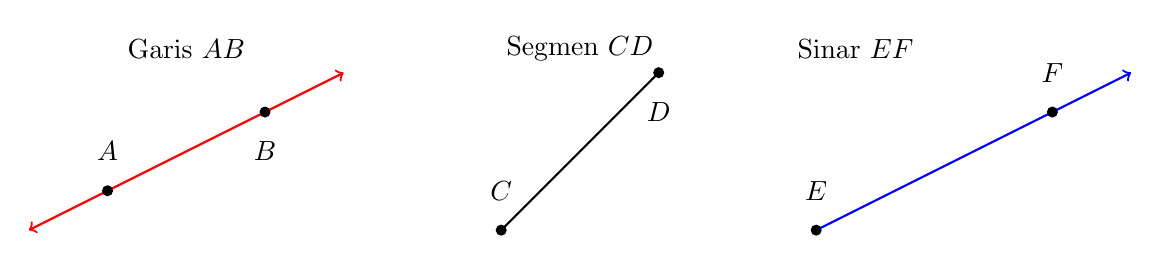
\begin{tikzpicture}
    % Draw a line
    \draw[red, thick, <->] (-4,-1) -- (0,1);
    \node at (-2,1.3) {Garis $AB$};
    \fill (-3,-0.5) circle (2pt);
    \fill (-1,0.5) circle (2pt);
    \node at (-3,-0) {$A$};
    \node at (-1,0) {$B$};

    % Draw a segment
    \draw[thick] (2,-1) -- (4,1);
    \node at (3,1.3) {Segmen $CD$};
    \fill (2,-1) circle (2pt);
    \fill (4,1) circle (2pt);
    \node at (2,-0.5) {$C$};
    \node at (4,0.5) {$D$};

    % Draw a ray
    \draw[blue, thick, ->] (6,-1) -- (10,1);
    \node at (6.5,1.3) {Sinar $EF$};
    \fill (6,-1) circle (2pt);
    \fill (9,0.5) circle (2pt);
    \node at (6,-0.5) {$E$};
    \node at (9,1) {$F$};
\end{tikzpicture}
\end{center}